\tikzstyle{startstop} = [rectangle, rounded corners,
minimum width=3cm,
minimum height=1cm,
text centered,
draw=black,
fill=red!30]

\definecolor{icscolor}{RGB}{31,119,180}
\definecolor{seccolor}{RGB}{255,127,14}
\definecolor{thirdcolor}{RGB}{44,160,44}

\tikzstyle{ics} = [rectangle, rounded corners,
minimum width=1cm,
minimum height=1cm, text centered,
draw=black, text=white, fill=icscolor]

\tikzstyle{sec} = [rectangle, rounded corners,
minimum width=1cm,
minimum height=1cm, text centered,
draw=black, fill=seccolor]

\tikzstyle{study} = [rectangle,
rounded corners,
minimum width=1cm,
minimum height=1cm,
text centered,
draw=black,
fill=thirdcolor, text=white]

\tikzstyle{decision} = [diamond,
minimum width=3cm,
minimum height=1cm,
text centered,
draw=black,
fill=green!30]
\tikzstyle{arrow} = [thick,->,>=stealth]


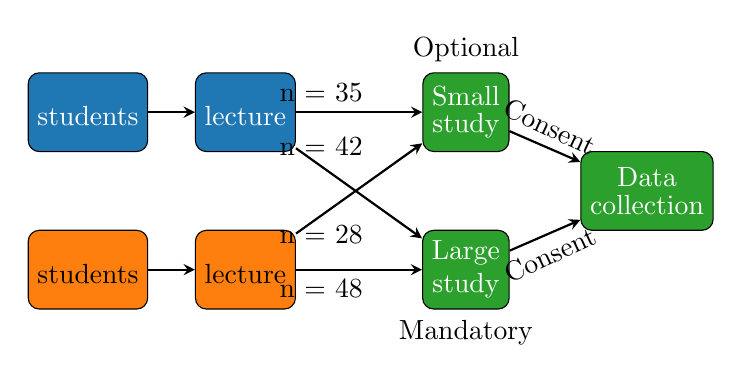
\begin{tikzpicture}[node distance=2cm]

    \node (ics1) [ics] {\shortstack{\ICS\\students} };
    \node (sec1) [sec, below of=ics1] {\shortstack{\SEC\\students} };
    \node (ics2) [ics, right of=ics1] {\shortstack{\ICS\\lecture} };
    \node (sec2) [sec, right of=sec1] {\shortstack{\SEC\\lecture} };
    \node (ss) [study, right of=ics2, xshift=0.8cm] {\shortstack{Small\\study} };
    \node (ls) [study, right of=sec2, xshift=0.8cm] {\shortstack{Large\\study} } ;
    \node [above of=ss, yshift=-1.2cm] {Optional};
    \node [below of=ls, yshift=1.2cm] {Mandatory};
    \node (data) [study, right of=ss, xshift=0.3cm, yshift=-1cm] {\shortstack{Data\\collection} } ;



    \draw [arrow] (ics1) -- (ics2);
    \draw [arrow] (sec1) -- (sec2);
    % \draw [arrow] (ics2) -- node[anchor=south] {Optional} node[anchor=north,pos=0.2] {35}  (ss);
    % \draw [arrow] (ics2) -- node[anchor=north,pos=0.1] {42}  (ls);
    % \draw [arrow] (sec2) -- node[anchor=south,pos=0.1] {28} (ss);
    % \draw [arrow] (sec2) -- node[anchor=north] {Mandatory} node[anchor=south,pos=0.2] {48} (ls);
\draw [arrow] (ics2) -- node[anchor=south,pos=0.2] {$\text{ }$$\text{ }$$\text{ }$$\text{ }$n = 35}  (ss);
\draw [arrow] (sec2) --  node[anchor=north,pos=0.2] {$\text{ }$$\text{ }$$\text{ }$$\text{ }$n = 48} (ls);
\draw [arrow] (ics2) -- node[anchor=south,pos=0.2] {$\text{ }$$\text{ }$$\text{ }$$\text{ }$n = 42}  (ls);
\draw [arrow] (sec2) -- node[anchor=north,pos=0.2] {$\text{ }$$\text{ }$$\text{ }$$\text{ }$n = 28} (ss);
    \draw [arrow] (ss) -- node[anchor=south,pos=0.45, rotate=-25] {Consent} (data);
    \draw [arrow] (ls) -- node[anchor=north,pos=0.45, rotate=25] {Consent} (data);


\end{tikzpicture}